\newcommand{\x}{\mathbf{x}}
\newcommand{\w}{\mathbf{w}}
\documentclass[thesis.tex]{subfiles}
\begin{document}

\chapter{Pedestrian detection}
\label{sec:od}
In this chapter we describe the pedestrian detection problem and how we apply our descriptor to solve it.

Object detection is the problem of locating specified objects in images. One application of this is pedestrian detection, which we have decided to focus on as it is simple and has extensive datasets. A common approach to object detection is to extract regions from the image, reducing the problem to binary classification of the presence of the specified object in each region. Using this approach, we are able to compute one descriptor for each region. We furthermore assume fixed size regions in scale-space, allowing us to directly compare our descriptors. The classification of pedestrians is done using a linear SVM.

The chapter is structured as follows...

\section{Support vector machine}

Suppose we have some training data split into positive and negative elements. In our case these are $d$-dimensional descriptors of regions with and without pedestrians. We wish to construct a binary classifier which accurately assigns a classification score denoting how confident we are that there is or isn't a pedestrian present. The approach of a linear support vector machine (SVM) is to place a $(d-1)$-dimensional hyperplane in descriptor space which separates the two classes. The hyperplane $(\w,b)$ is defined as the points $\x$ satisfying
%
\begin{align*}
\w \cdot \x - b = 0.
\end{align*}
%
If the data is linearly separable, we can search for the \emph{maximum-margin} hyperplane defined as having the largest possible distance to the nearest point of each class. This distance defines the margin. Formally, this can be written as the constrained optimization problem
%
\begin{align*}
\min_{\w,b} \frac12 \| \w \|^2 \qquad \text{subject to} \qquad y_i (\w \cdot \x_i - b) \geq 1,
\end{align*}
%
where $\x_i$ are training data points and $y_i \in \{-1,1\}$ their respective condition labels.

However, linear separation of the two classes is almost never feasible. Instead a \emph{soft-margin} SVM is used. The idea is to allow some of the data points to be placed on the wrong side of the margin. The total distance of misplaced points to the margin is minimized, in addition to maximizing the margin. This is done by introducing a \emph{cost} parameter $C$ which weights the importance of the misplacement minimization relative to the margin maximization. Formally, the soft-margin optimization problem is written as
%
\begin{align*}
\min_{\w,\boldsymbol{\xi},b} \left\{ \frac12 \| \w \|^2 + C \sum_i \xi_i \right\} \qquad \text{subject to} \qquad \begin{aligned} y_i (\w \cdot \x_i - b) &\geq 1 - \xi_i, \\ \xi_i &\geq 0, \end{aligned}
\end{align*}
%
where $\xi_i$ are slack variables allowing for misplaced points.

Mention separate costs for each class.

We use the $L_2$-regularized $L_2$ loss support vector classifier from LIBLINEAR v. 1.94 \cite{fan2008liblinear}

\section{Performance measures}

\section{Dataset}
\label{sec:odDataset}

The dataset we use for training and testing our descriptor on the pedestrian detection application is called the \emph{INRIA Person Dataset}\footnote{\url{http://pascal.inrialpes.fr/data/human/}} (from now on called the INRIA dataset) constructed by \citet{dalal2005histograms}.

It consists of various real world images grouped into two subsets: Images with pedestrians (positives) and images without pedestrians (negatives). The positive images are rescaled cutouts centered around each pedestrian in larger images. The cutouts are first extracted and then individually re-scaled to make the pedestrian of each cutout 96 pixels in height from their feet to shoulders. The size of the cutouts are $64 \times 128$ pixels with a 3 pixel border to avoid boundary condition effects. In case a pedestrian cutout is smaller than the defined size after resizing, the borders are replicated to achieve the desired dimensions.
The positive set only contains images of somewhat upright persons that initially were at least 100 pixels in height. In order to improve the robustness of the dataset against reflected images, each positive cutout has its horizontally flipped image included as well.

The training dataset has a total of 2416 positives and 1218 negative images.
The test dataset has a total of 1126 positives and 453 negative images.

\Cref{fig:inriaExampleImages} shows examples of positive \subref{fig:inriaPositives} and negative \subref{fig:inriaNegatives} images from the INRIA dataset. From the positive examples we clearly see the high variety of upright positions and surroundings in the dataset.

\begin{figure}
	\centering
	\begin{subfigure}[t]{\textwidth}
		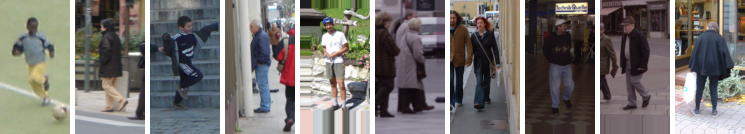
\includegraphics[width=\textwidth]{img/inriaPositives.png}
		\caption{Positives}
		\label{fig:inriaPositives}
		\vspace{2mm}
	\end{subfigure}
	\begin{subfigure}[t]{\textwidth}
		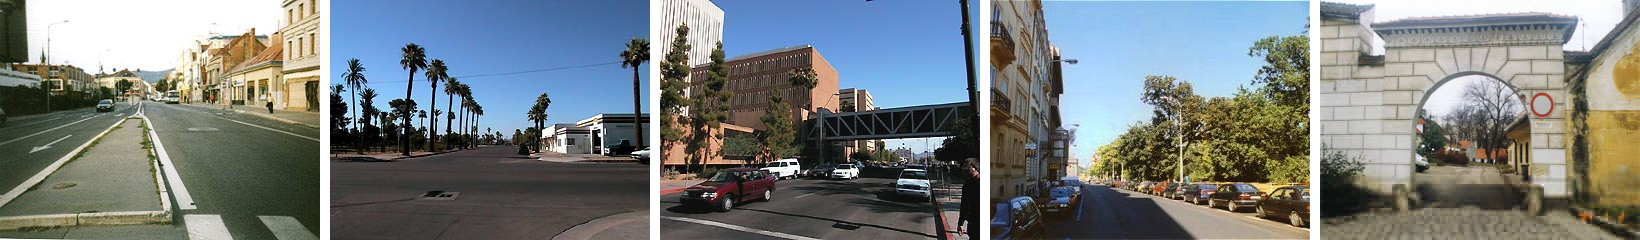
\includegraphics[width=\textwidth]{img/inriaNegatives.png}
		\caption{Negatives}
		\label{fig:inriaNegatives}
	\end{subfigure}
	\caption{Example INRIA images.}
	\label{fig:inriaExampleImages}
\end{figure}

\subsection{Pitfalls and deficiencies}
We have found two smaller problems with the INRIA dataset which could affect the results of using the dataset. The first problem is duplicate images. Amongst the negative training images we have found 10 pair-wise duplicates. This chould bias the svm since it effectively means that these images are weighted twice as high as the others. Given the small percentage of duplicates in the dataset the effect should however be close to nothing. In the initial training there are furthermore extracted windows at different random positions of the duplicates which decreases the bias even more. We have likewise found one duplicated image in the negative test set.

The second problem is the presence of people in some of the negatives.
\Cref{fig:inriaNegativePersons} show two examples of persons in the negative images of the INRIA dataset. The people are however either too small to fit correctly into the sliding window at any of the used scales or partially occluded by the image bounds to such an extent that we shouldn't be able to detect them anyway.

\begin{figure}[tb]
	\begin{subfigure}[t]{0.5\textwidth}
		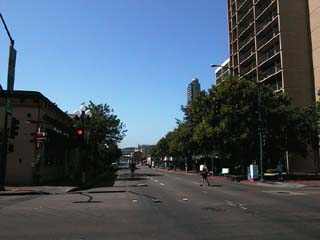
\includegraphics[width=\textwidth]{img/inriaManExample1.png}
	\end{subfigure}
	\begin{subfigure}[t]{0.5\textwidth}
		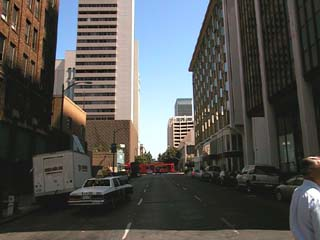
\includegraphics[width=\textwidth]{img/inriaManOccluded.png}
	\end{subfigure}
	\caption{Examples of persons in negative images}
	\label{fig:inriaNegativePersons}
\end{figure}

\section{Test setup}
%
We have a test setup for parameter optimization using only the training data, and a more involved test setup for evaluating descriptors on test data.

Our parameter optimization setup is as follows. The training data is split into six parts, for the purpose of (leave-one-out) cross-validation by training on five parts and training on one. For each split, an SVM is trained and evaluated.

Notes:

We follow \citet{dalal2005histograms}

Initial training: X randomly chosen windows per negative image and all positives
Hard training: Predict on sliding window of negatives ~ 2.2 million windows. Add hard negatives to training set and re-train.

Sliding window: 10 pixel in between windows. Multiscale.

Test on test set with sliding window on negatives ~ 1 million windows.

\section{Example}

\begin{figure}
	\centering
	\begin{subfigure}[t]{0.3\textwidth}
		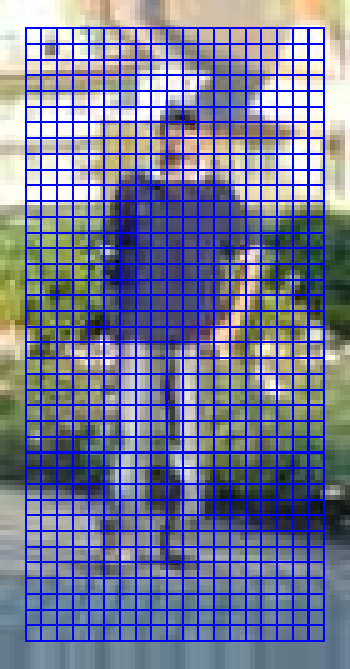
\includegraphics[width=\textwidth]{img/inriaExampleCells.pdf}
		\caption{}
		\label{fig:inriaExampleCells}
		\vspace{2mm}
	\end{subfigure}
	\begin{subfigure}[t]{0.3\textwidth}
		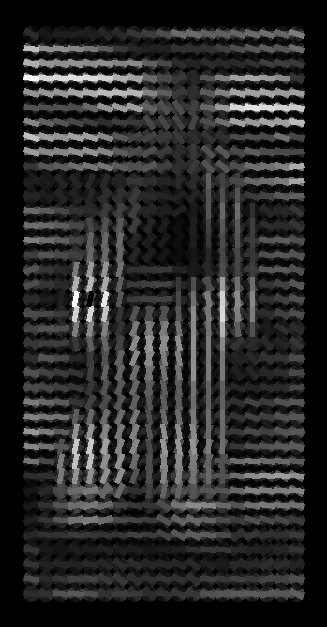
\includegraphics[width=\textwidth]{img/inriaExampleDescriptor.pdf}
		\caption{}
		\label{fig:inriaExampleDescriptor}
		\vspace{2mm}
	\end{subfigure}
	\begin{subfigure}[t]{0.3\textwidth}
		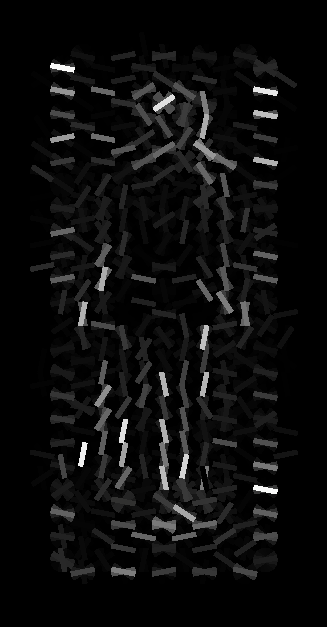
\includegraphics[width=\textwidth]{img/inriaExampleDescriptorSvm.pdf}
		\caption{}
		\label{fig:inriaExampleDescriptorSvm}
		\vspace{2mm}
	\end{subfigure}
	\caption{Example stuff.}
	\label{fig:imageCorrespondenceCurves}
\end{figure}

\begin{figure}
	\centering
	\begin{subfigure}[t]{\textwidth}
		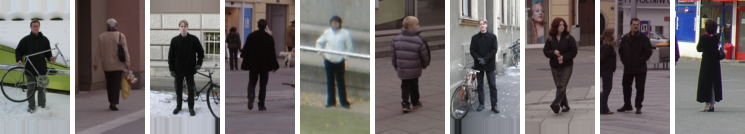
\includegraphics[width=\textwidth]{img/objectDetectionTP.png}
		\caption{True positives}
		\label{fig:objectDetectionTP}
		\vspace{2mm}
	\end{subfigure}
	\begin{subfigure}[t]{\textwidth}
		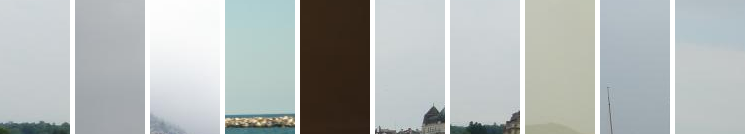
\includegraphics[width=\textwidth]{img/objectDetectionTN.png}
		\caption{True negatives}
		\label{fig:objectDetectionTN}
		\vspace{2mm}
	\end{subfigure}
	\begin{subfigure}[t]{\textwidth}
		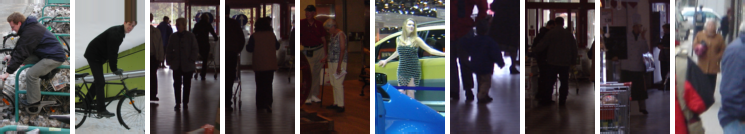
\includegraphics[width=\textwidth]{img/objectDetectionFN.png}
		\caption{False negatives}
		\label{fig:objectDetectionFN}
		\vspace{2mm}
	\end{subfigure}
	\begin{subfigure}[t]{\textwidth}
		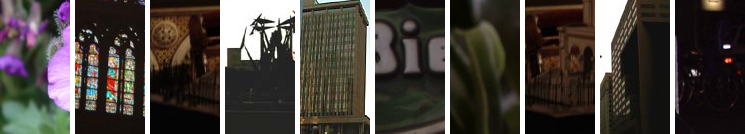
\includegraphics[width=\textwidth]{img/objectDetectionFP.png}
		\caption{False positives}
		\label{fig:objectDetectionFP}
	\end{subfigure}
	\caption{Example classifications of INRIA windows.}
	\label{fig:imageCorrespondenceCurves}
\end{figure}

\section{Parameter study}
\label{sec:odParameterStudy}

\subbibliography

\end{document}
